\documentclass[xcolor=dvipsname]{beamer} %handout, ignorenonframetext

%\usepackage[ngerman]{babel}
\usepackage[utf8]{inputenc}
\usepackage{amsmath}
\usepackage{graphicx}
\usepackage{subfigure}
\usepackage{multimedia}
\usepackage{wrapfig}
\usepackage{listings}
\usepackage{comment}
\usepackage{framed,color}
\usepackage{listings}


\fboxsep=1pt%padding thickness
\fboxrule=1pt%border thickness
\usepackage{fancybox}

\usepackage{lipsum}
\usepackage{tabularx}
\usepackage{colortbl}
\usepackage{url}


\hypersetup{
	linkcolor=DarkSkyBlue,
	citecolor= DarkSkyBlue,
	filecolor= DarkSkyBlue,
	urlcolor= DarkSkyBlue
}


% COLOR-DEFINITION
%%%%%%%%%%%%%%%%%%%%%%%%
\definecolor{LightButter}{rgb}{0.98,0.91,0.31}
\definecolor{LightOrange}{rgb}{0.98,0.68,0.24}
\definecolor{LightChocolate}{rgb}{0.91,0.72,0.43}
\definecolor{LightChameleon}{rgb}{0.54,0.88,0.20}
\definecolor{LightSkyBlue}{rgb}{0.45,0.62,0.81}
\definecolor{LightPlum}{rgb}{0.68,0.50,0.66}
\definecolor{LightScarletRed}{rgb}{0.93,0.16,0.16}
\definecolor{LightGray}{rgb}{0.80,0.80,0.80}
\definecolor{Butter}{rgb}{0.93,0.86,0.25}
\definecolor{Orange}{rgb}{0.96,0.47,0.00}
\definecolor{Chocolate}{rgb}{0.75,0.49,0.07}
\definecolor{Chameleon}{rgb}{0.45,0.82,0.09}
\definecolor{SkyBlue}{rgb}{0.20,0.39,0.64}
\definecolor{Plum}{rgb}{0.46,0.31,0.48}
\definecolor{ScarletRed}{rgb}{0.80,0.00,0.00}
\definecolor{DarkButter}{rgb}{0.77,0.62,0.00}
\definecolor{DarkOrange}{rgb}{0.80,0.36,0.00}
\definecolor{DarkChocolate}{rgb}{0.56,0.35,0.01}
\definecolor{DarkChameleon}{rgb}{0.30,0.60,0.02}
\definecolor{DarkSkyBlue}{rgb}{0.12,0.29,0.53}
\definecolor{DarkPlum}{rgb}{0.36,0.21,0.40}
\definecolor{DarkScarletRed}{rgb}{0.64,0.00,0.00}



% HPI-THEME
%%%%%%%%%%%%%%%%%%%%%%%%
\RequirePackage{scrlfile}
%\ReplaceFile{beamerthemehpiswa.sty}{theme/beamerthemehpiswa.sty}
%\ReplaceFile{beamercolorthemehpiswa.sty}{theme/beamercolorthemehpiswa.sty}
%\ReplaceFile{beamerfontthemehpiswa.sty}{theme/beamerfontthemehpiswa.sty}
%\ReplaceFile{beamerinnerthemehpiswa.sty}{theme/beamerinnerthemehpiswa.sty}
%\ReplaceFile{beamerouterthemehpiswa.sty}{theme/beamerouterthemehpiswa.sty}
%\ReplaceFile{hpi.png}{theme/hpi.png}
\usetheme{hpiswa}


% BEAMER-Anpassungen
%%%%%%%%%%%%%%%%%%%%%%%%
\setbeamercolor{block title}{bg=DarkOrange}
\setbeamercolor{block body}{bg=Orange!20}
%\setbeamercolor{block title alerted}{bg=red}
\setbeamercolor{block body alerted}{bg=red!20}
%\setbeamercolor{block title example}{bg=green}
\setbeamercolor{block body example}{bg=DarkChameleon!20}
%\usecolortheme[RGB={205,173,0}]{structure}
\usecolortheme[RGB={30,74,135}]{structure}

\usecolortheme{orchid}
%\usefonttheme{professionalfonts}
%\useoutertheme[subsection=false]{smoothbars}
%\useinnertheme{rectangles}
%\setbeamertemplate{blocks}[shadow=true]

\setbeamercovered{transparent}
\setbeamertemplate{navigation symbols}{}%remove navigation symbols



% Eigene Anpassungen
%%%%%%%%%%%%%%%%%%%%

% Explainframes:
\usepackage{ifthen}
\newboolean{isexplainframe}
\setboolean{isexplainframe}{false}
\mode<handout>{
\newenvironment{explainframe}[1]{
\setboolean{isexplainframe}{true}
\addtocounter{framenumber}{-1}
\setbeamertemplate{background}[grid][step=5mm,color=LightGray]
\begin{frame}[fragile,environment=explainframe]{Handout only: #1}%
}{%
\end{frame}%
\setboolean{isexplainframe}{false}
}
\newenvironment{clearexplainframe}[0]{
\setboolean{isexplainframe}{true}
\addtocounter{framenumber}{-1}
\setbeamertemplate{background}[grid][step=5mm,color=LightGray]
\begin{frame}[fragile,environment=clearexplainframe]%
}{%
\end{frame}%
\setboolean{isexplainframe}{false}
}
}
\mode<beamer>{
\excludecomment{explainframe}
\excludecomment{clearexplainframe}
}

\setbeamertemplate{footline}{%
	\leavevmode%
	\hbox{%
		\begin{beamercolorbox}[wd=.45\paperwidth,ht=2.25ex,dp=1ex,center]{author in head/foot}%
			\usebeamerfont{author in head/foot}\insertinstitute
		\end{beamercolorbox}%
		\begin{beamercolorbox}[wd=.2\paperwidth,ht=2.25ex,dp=1ex,center]{title in head/foot}%
			\usebeamerfont{title in head/foot}\insertshorttitle
		\end{beamercolorbox}%
		\begin{beamercolorbox}[wd=.35\paperwidth,ht=2.25ex,dp=1ex,right]{date in head/foot}%
			\usebeamerfont{date in head/foot}\insertshortdate{}\hspace*{2em}
			\insertframenumber{}\ifthenelse{\boolean{isexplainframe}}{E}{} / \inserttotalframenumber\hspace*{2ex}
	\end{beamercolorbox}}%
	\vskip0pt%
}

\definecolor{javared}{rgb}{0.6,0,0} % for strings
\definecolor{javagreen}{rgb}{0.25,0.5,0.35} % comments
\definecolor{javapurple}{rgb}{0.5,0,0.35} % keywords
\definecolor{javadocblue}{rgb}{0.25,0.35,0.75} % javadoc

\lstset{
  language=Ruby,
  basicstyle=\normalsize\ttfamily,
  keywordstyle=\color{javapurple}\bfseries,
  stringstyle=\color{javared},
  commentstyle=\color{javagreen},
  morecomment=[s][\color{javadocblue}]{/**}{*/},
  tabsize=4,
  showspaces=false,
  showstringspaces=false,
  breaklines=true
}


% Gliederung vor jedem Punkt:
\AtBeginSection[]{
\ifthenelse{\equal{\value{section}}{1}}{}{
\ifthenelse{\equal{\value{section}}{6}}{}{
\begin{frame}{Overview}
	\tableofcontents[currentsection, hideothersubsections]
\end{frame}
}
}
}


% Quote-Environment:

\renewenvironment{quote}{%
\begin{exampleblock}{}%
\begin{center}%
\begin{large}%
``}{%
''\end{large}%
\end{center}%
\end{exampleblock}}




% Dokument-Meta-Daten:
%%%%%%%%%%%%%%%%%%%%%%%
\title{Call-target-specific Method Arguments}
\subtitle{ICOOOLPS 2015}
\author{Fabio Niephaus, Matthias Springer, Tim Felgentreff, Tobias Pape, Robert Hirschfeld}
\date{July 6, 2015}
\institute[2012]{Hasso Plattner Institute, Software Architecture Group}



\begin{document}

\begin{frame}[plain]
	\maketitle
\end{frame}
\begin{frame}{Overview}
	\tableofcontents[hideallsubsections]
\end{frame}

\section{Introduction}
\begin{frame}{Introduction}
	\begin{itemize}
		\item \textbf{Goal:} Make argument handling faster $\rightarrow$ make method calls faster
		\item \textbf{How to:} Prepare arguments at call site.
		\item \textbf{Running example:} Keyword arguments in JRuby $\rightarrow$ twice as fast
	\end{itemize}

	\begin{table}
		\centering
		
\includegraphics[width=0.5\textwidth]{jruby.png} \qquad \qquad
		
\includegraphics[width=0.2\textwidth]{truffle.jpg}
	\end{table}
\end{frame}

\section{Concept}
\begin{frame}[fragile]{Argument Mismatch}
\begin{table}
	\centering
	\textbf{Method Signature Parameters $\not=$ Call Arguments}
\end{table}

\begin{table}
\begin{minipage}{0.8\textwidth}
\begin{lstlisting}
def method(a: 0, b: 0, c: 0)
  ...
end

method(a: 1, b: 2, c: 3)

method(b: 1, a: 2)
method(c: 4)
method()
\end{lstlisting}
\end{minipage} % comment
\begin{minipage}{0.45\textwidth}
%\emph{signature:} \texttt{(a, b, c)} \\ \\ \\ \\
%\emph{arguments:} \texttt{(a, b, c)} \\ \\
%\emph{arguments:} \texttt{(b, a)} \\ 
%\emph{arguments:} \texttt{(c)} \\ 
%\emph{arguments:} \texttt{($\emptyset$)} \\
\end{minipage}
\end{table}
\end{frame}

\begin{frame}{When to Convert Arguments?}
\begin{minipage}{0.49\textwidth}
\begin{table}
\centering
\textbf{Convert after invoke:} \newline \newline
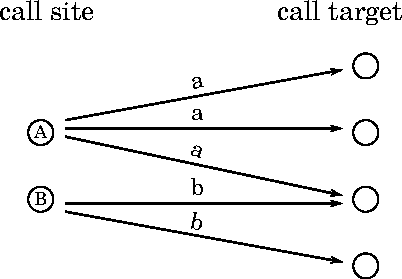
\includegraphics[width=0.8\textwidth]{pic_regular.pdf}
\end{table}
\end{minipage} % comment
\begin{minipage}{0.49\textwidth}
\begin{table}
\centering
\textbf{Convert before invoke:} \newline \newline
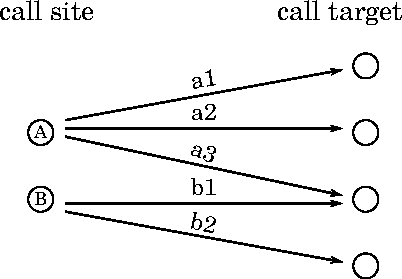
\includegraphics[width=0.8\textwidth]{pic_calltarget.pdf}
\end{table}
\end{minipage}
\end{frame}

\begin{frame}{When to Convert Arguments?}
\begin{minipage}{0.49\textwidth}
\begin{table}
\centering
\textbf{Convert after invoke:} \newline \newline
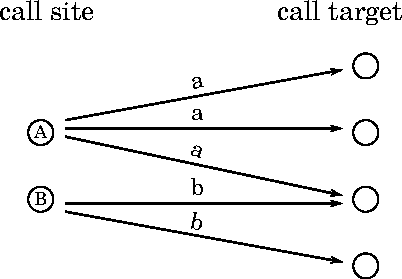
\includegraphics[width=0.8\textwidth]{pic_regular.pdf}
\end{table}
\begin{enumerate}
	\item Convert args to generic repres.
	\item Lookup receiver
	\item Invoke target method
	\item Convert args to specific repres.
\end{enumerate}
\end{minipage} % comment
\begin{minipage}{0.49\textwidth}
\begin{table}
\centering
\textbf{Convert before invoke:} \newline \newline
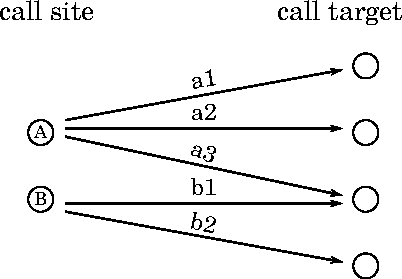
\includegraphics[width=0.8\textwidth]{pic_calltarget.pdf}
\end{table}
\begin{enumerate}
	\item Lookup receiver
	\item Convert args to specific repres.
	\item Invoke target method \newline
\end{enumerate}
\end{minipage}
\end{frame}

\section{Example: Ruby Keyword Arguments}
\begin{frame}[fragile]{Convert After Invocation: Call-site-specific Arguments}
\begin{minipage}{0.25\textwidth}
\centering
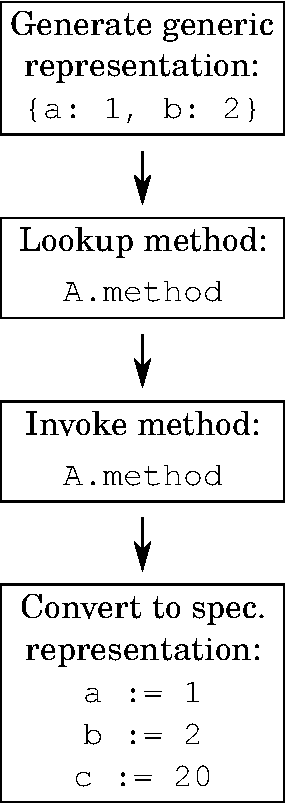
\includegraphics[height=0.8\textheight]{convert_after.pdf}
\end{minipage} % comment
\begin{minipage}{0.7\textwidth}
\begin{lstlisting}
def A.method(b: 10, c: 20, a: 30)
  ...
end

obj.method(a: 1, b: 2)
\end{lstlisting}
\end{minipage}
\end{frame}

\begin{frame}[fragile]{Convert Before Invocation: Call-target-specific Arguments}
\begin{minipage}{0.3\textwidth}
\centering
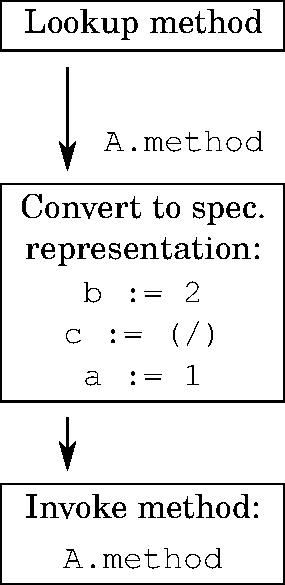
\includegraphics[height=0.6\textheight]{convert_before.pdf}
\end{minipage} % comment
\begin{minipage}{0.65\textwidth}
\begin{lstlisting}
def A.method(b: 10, c: 20, a: 30)
  ...
end

obj.method(a: 1, b: 2)
\end{lstlisting}
\end{minipage}
\end{frame}


\begin{frame}[fragile]{Convert Before Invocation: Call-target-specific Arguments}
\begin{minipage}{0.55\textwidth}
\centering
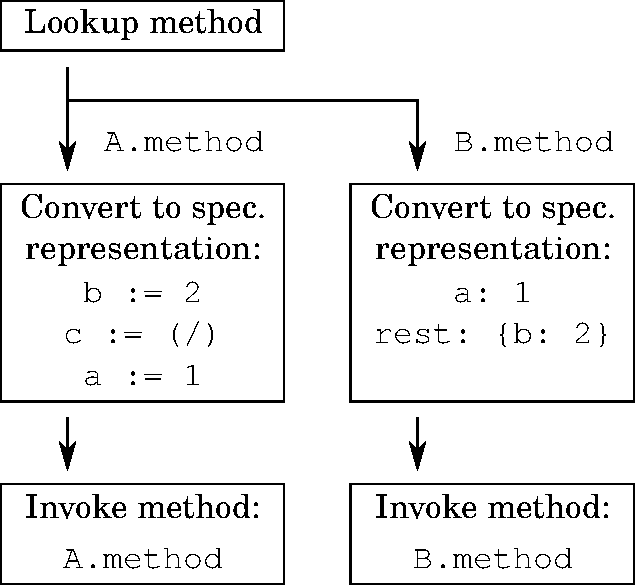
\includegraphics[height=0.6\textheight]{convert_before2.pdf}
\end{minipage} % comment
\begin{minipage}{0.4\textwidth}
\begin{lstlisting}
def A.method(b: 10, c: 20, a: 30)
  ...
end

def B.method(a:, **rest)
  ...
end

obj.method(a: 1, b: 2)
\end{lstlisting}
\end{minipage}
\end{frame}

\begin{frame}[fragile]{Convert Before Invocation: Call-target-specific Arguments}
\begin{minipage}{0.7\textwidth}
\centering
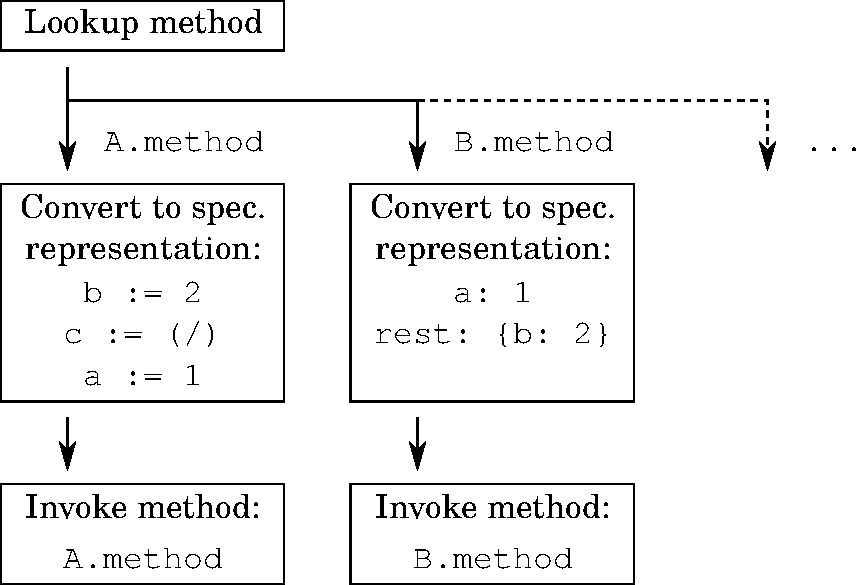
\includegraphics[height=0.6\textheight]{convert_before3.pdf}
\end{minipage} % comment
\begin{minipage}{0.25\textwidth}

\end{minipage}
\end{frame}

\begin{frame}{Call-target-specific Method Arguments}
\begin{itemize}
	\item Code/AST for generating arguments representation depends on call target.
	\item We cache one AST subtree generating the arguments array per PIC entry.
	\item Call-target-specific argument handling is part of the PIC.
\end{itemize}
\end{frame}

\section{Implementation Details}
\begin{frame}{PIC Argument Cache}
\begin{itemize}
	\item Truffle: AST Interpreter Framework.
	\item PIC is implemented as linked list of AST nodes.
	\item We cache one AST subtree generating the array of arguments per PIC entry. No bytecode manipulations neccessary.
\end{itemize}
\end{frame}

\begin{frame}[fragile]{Execution Order of Argument Nodes}
\begin{minipage}{0.45\textwidth}
\begin{lstlisting}
def meth(a: 0, b: 0)
  ...
end
\end{lstlisting}
\end{minipage} % comment
\begin{minipage}{0.5\textwidth}
\begin{lstlisting}
meth(b: foo(), a: bar())
\end{lstlisting}
\end{minipage}

\begin{table}
\centering
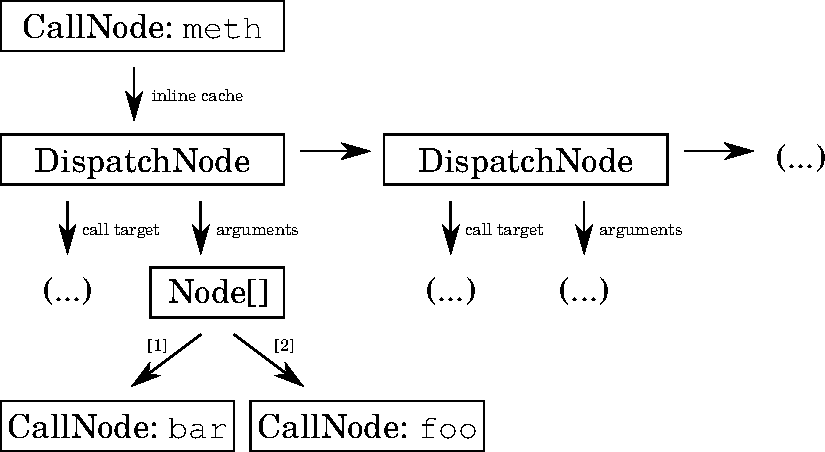
\includegraphics[width=0.8\textwidth]{ast_nodes.pdf}
\end{table}
\end{frame}

\begin{frame}{Megamorphic Call Sites}
\begin{itemize}
	\item Call site switches to \emph{megamorphic} once the PIC treshold is reached.
	\item Megamorphic call sites use call-site-specific method argument \\ (old behavior).
	\item Call target is able to detect whether call is \emph{optimized} (call-target-specific args) or \emph{unoptimized} (call-site-specific args).
\end{itemize}
\end{frame}

\section{Benchmarks}
\begin{frame}{Micro-Benchmarks}
	\centering
	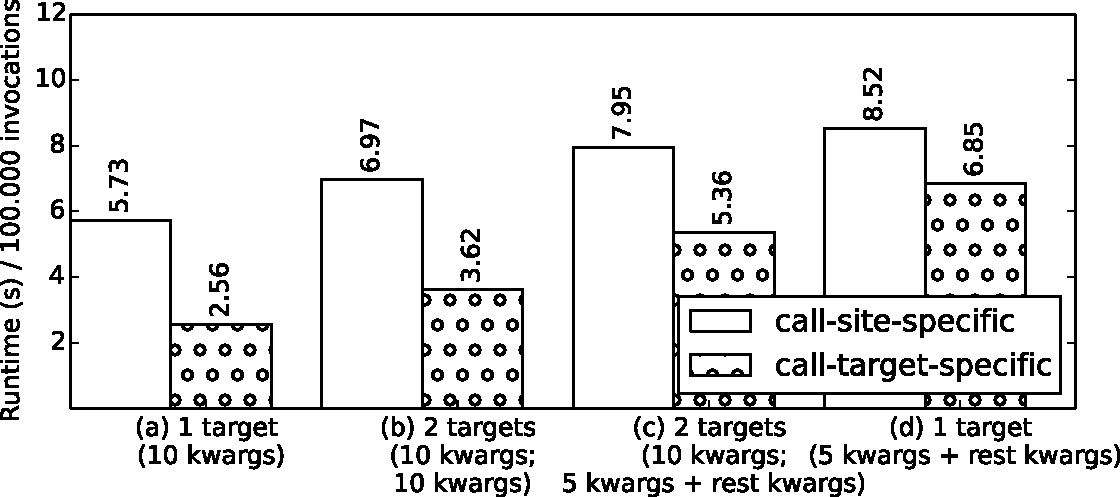
\includegraphics[width=\textwidth]{benchmark.pdf}
\end{frame}

\section{Summary}
\begin{frame}{Summary}
\begin{itemize}
	\item Call-site-specific method arguments: an \textbf{optimization for method argument handling} in dynamically-typed languages.
	\item Call sites can have multiple polymorphic call targets.
	\item \textbf{Prepare arguments} for call target at call site.
	\item Only efficient if \textbf{call target analysis is cached} at the call site \\ (as part of the PIC).
\end{itemize}
\end{frame}

\section{Related Work}
\begin{frame}[fragile]{MagLev}
\begin{minipage}{0.15\textwidth}
\centering

\includegraphics[width=0.9\textwidth]{maglev-logo.png}
\end{minipage} %comment
\begin{minipage}{0.8\textwidth}
\begin{itemize}
	\item MagLev: a Ruby implementation in Smalltalk (GemStone/S).
	\item Compiled to byte code for a Smalltalk virtual machine
	\item Generates a number of wrapper (\emph{bridge}) methods for different method arguments.
\end{itemize}
\end{minipage}

\begin{lstlisting}
def method(a, b = 1, *args)
...
end

def method#1(a)
	# call method(a, 1)
end

def method#3(a, b, c, d, e)
	# call method(a, b, [c, d, e])
end
\end{lstlisting}
\end{frame}
\end{document}
